\documentclass[aspectratio=169,t]{beamer}

\usetheme{default}
\usecolortheme{default}

\definecolor{darkblue}{RGB}{15,40,80}
\definecolor{midblue}{RGB}{30,80,160}
\definecolor{lightblue}{RGB}{200,220,245}
\definecolor{accent}{RGB}{220,80,40}
\definecolor{dkgreen}{RGB}{30,130,70}
\definecolor{gold}{RGB}{180,140,0}
\definecolor{lightgray}{RGB}{240,242,246}
\definecolor{purple}{RGB}{120,40,160}

\setbeamercolor{frametitle}{fg=white,bg=darkblue}
\setbeamercolor{title}{fg=white}
\setbeamercolor{subtitle}{fg=lightblue}
\setbeamercolor{author}{fg=lightblue}
\setbeamercolor{normal text}{fg=darkblue}
\setbeamercolor{block title}{fg=white,bg=midblue}
\setbeamercolor{block body}{fg=darkblue,bg=lightblue!40}
\setbeamercolor{alerted text}{fg=accent}
\setbeamercolor{example text}{fg=dkgreen}
\setbeamercolor{structure}{fg=midblue}
\setbeamercolor{itemize item}{fg=accent}
\setbeamercolor{itemize subitem}{fg=midblue}
\setbeamercolor{enumerate item}{fg=accent}

\setbeamerfont{frametitle}{size=\large,series=\bfseries}
\setbeamerfont{title}{size=\LARGE,series=\bfseries}
\setbeamerfont{block title}{series=\bfseries}

\setbeamertemplate{navigation symbols}{}
\setbeamertemplate{itemize item}{\small\raise0.5pt\hbox{$\bullet$}}
\setbeamertemplate{itemize subitem}{\small\raise0.5pt\hbox{$\circ$}}
\setbeamertemplate{frametitle}[default][center]
\setbeamertemplate{footline}{%
  \hfill\usebeamerfont{footline}\color{darkblue!50}%
  \insertframenumber/\inserttotalframenumber\hspace{4pt}\vspace{4pt}}

\usepackage{amsmath,amssymb}
\usepackage{booktabs}
\usepackage{xcolor}
\usepackage{colortbl}
\usepackage{tikz}
\usetikzlibrary{arrows.meta,positioning,shapes.geometric,fit,backgrounds,calc,decorations.pathreplacing}
\usepackage{pgfplots}
\pgfplotsset{compat=1.16}
\usepackage{array}

\newcommand{\pw}{\mathrm{pw}}
\newcommand{\tw}{\mathrm{tw}}
\newcommand{\Bell}{\mathrm{Bell}}
\newcommand{\nb}{n_{\mathrm{back}}}
\newcommand{\Gn}{G_n}

\title{Counting Hamiltonian Paths\\in Square-Sum Graphs}
\subtitle{Talk I: Algorithms and Combinatorics}
\author{Victor S.\ Miller}
\date{}

\begin{document}

% ==================== TITLE ====================
{
\setbeamercolor{background canvas}{bg=darkblue}
\begin{frame}[plain]
  \vspace{1.0cm}
  \begin{center}
    {\color{lightblue}\small\itshape Talk I of II}\\[0.5cm]
    {\color{white}\LARGE\bfseries Counting Hamiltonian Paths\\[4pt]
     in Square-Sum Graphs}\\[0.7cm]
    {\color{lightblue}\large Algorithms and Combinatorics}\\[0.9cm]
    {\color{white}\large Victor S.\ Miller}\\[0.3cm]
    {\color{lightblue!70}\normalsize \today}
  \end{center}
\end{frame}
}

% ==================== OUTLINE ====================
\begin{frame}{Talk Outline}
\begin{columns}[t]
\column{0.48\textwidth}
\textbf{\color{midblue}The Problem}
\begin{itemize}
  \item Square-sum graphs
  \item Hamiltonian paths: why hard?
\end{itemize}
\vspace{0.1cm}
\textbf{\color{midblue}Classical DP Foundations}
\begin{itemize}
  \item Bellman (1962), Held-Karp (1962)
  \item DP table structure
  \item Why ordering matters
  \item Pruning dead states (Z.\,H.~Du)
\end{itemize}
\vspace{0.1cm}
\textbf{\color{midblue}Bell Numbers and Pathwidth}
\begin{itemize}
  \item Bell numbers and state counts
  \item Vertex separation / pathwidth
  \item Fixed-parameter tractability
  \item Treewidth comparison
\end{itemize}

\column{0.48\textwidth}
\textbf{\color{midblue}Computing the Best Ordering}
\begin{itemize}
  \item MaxSAT for exact pathwidth
  \item Simulated annealing refinement
  \item Multi-start enumeration
  \item New: Kobayashi's DP
\end{itemize}
\vspace{0.3cm}
\textbf{\color{midblue}Practical Computation}
\begin{itemize}
  \item The record-merging bottleneck
  \item Competing approaches
\end{itemize}
\vspace{0.3cm}
\textbf{\color{midblue}New Results}
\begin{itemize}
  \item $|\mathrm{Ham}(G_n)|$ for $n\le 75$
  \item What comes next
\end{itemize}
\end{columns}
\end{frame}

% ==================== PART I: PROBLEM ====================
{
\setbeamercolor{background canvas}{bg=darkblue}
\begin{frame}[plain]
  \vspace{2cm}
  \begin{center}
    {\color{lightblue}\small Part I}\\[0.4cm]
    {\color{white}\LARGE\bfseries The Problem}
  \end{center}
\end{frame}
}

\begin{frame}{The Square-Sum Graph $G_n$}
\small
\begin{columns}[c]
\column{0.55\textwidth}
\begin{block}{Definition}
$G_n$ has vertices $\{1,\ldots,n\}$. Edge $(i,j)$ iff $i+j$ is a perfect square.
\end{block}

\vspace{0.2cm}
\begin{itemize}
  \item Connected for all $n \ge 15$; sparse (max degree $\approx 6$)
  \item Related to the recreational \emph{square-sum problem}
\end{itemize}

\vspace{0.2cm}
\textbf{Central question:}
How many \alert{undirected Hamiltonian paths} does $G_n$ contain?

\vspace{0.2cm}
\begin{alertblock}{Hardness}
Counting Hamiltonian paths is \textbf{\#P-complete} in general.\\
Brute force for $n=61$: $61! \approx 10^{83}$ orderings to check.
\end{alertblock}

\column{0.42\textwidth}
\begin{center}
\begin{tabular}{rr}
\toprule
$n$ & $|\mathrm{Ham}(G_n)|$ \\
\midrule
15 & 1 \\
17 & 1 \\
18--20 & 0 \\
25 & 10 \\
35 & 17{,}175 \\
45 & 12{,}220{,}138 \\
57 & 68{,}092{,}497{,}615 \\
61 & 3{,}711{,}439{,}128{,}718 \\
\rowcolor{dkgreen!15}
75 & 9{,}231{,}885{,}593{,}047{,}053{,}408 \\
\bottomrule
\end{tabular}
\end{center}
{\small\color{dkgreen} New values for $n\le 75$ (Part VI)}
\end{columns}
\end{frame}

% ==================== PART II: CLASSICAL DP ====================
{
\setbeamercolor{background canvas}{bg=darkblue}
\begin{frame}[plain]
  \vspace{2cm}
  \begin{center}
    {\color{lightblue}\small Part II}\\[0.4cm]
    {\color{white}\LARGE\bfseries Classical DP Foundations}
  \end{center}
\end{frame}
}

\begin{frame}{Historical Context: Bellman (1962) and Held-Karp (1962)}
\small
\begin{columns}[t]
\column{0.48\textwidth}
\begin{block}{Bellman (1962)}
  Dynamic programming for the Travelling Salesman Problem.
  State: $(S, v)$ where $S \subseteq V$ is the set of visited
  vertices and $v \in S$ is the current endpoint.\\[4pt]
  Recurrence:
  \[ C(S, v) = \min_{u \in S \setminus \{v\}} \bigl[C(S\setminus\{v\}, u) + d(u,v)\bigr] \]
  Time: $O(2^n \cdot n^2)$.  Space: $O(2^n \cdot n)$.
\end{block}

\column{0.48\textwidth}
\begin{block}{Held \& Karp (1962)}
  Independent discovery of the same approach; simultaneously
  showed that the DP dominates all previously known TSP algorithms
  and established $O(2^n \cdot n^2)$ as the complexity.\\[4pt]
  \textbf{Key insight:} the principle of optimality applies to
  Hamiltonian paths — a subpath must itself be optimal for its
  endpoint and visited set.
\end{block}
\end{columns}

\vspace{0.15cm}
\begin{center}
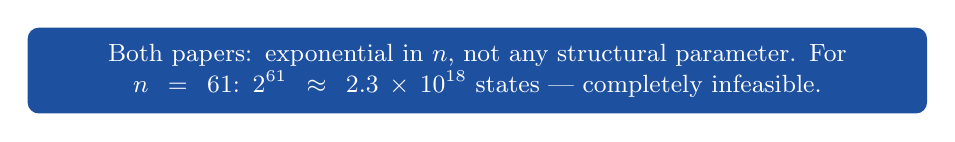
\begin{tikzpicture}
  \node[fill=midblue,rounded corners,text=white,inner sep=6pt,
        font=\small,text width=11cm,align=center]{
    Both papers: exponential in $n$, not any structural parameter.
    For $n=61$: $2^{61}\approx 2.3\times10^{18}$ states — completely infeasible.};
\end{tikzpicture}
\end{center}
\end{frame}

\begin{frame}{The Held-Karp DP Table Structure}
\begin{columns}[c]
\column{0.52\textwidth}
\textbf{State space} for Hamiltonian paths on $G_n$:
\begin{itemize}
  \item A state is a pair $(S, v)$: visited set $S \subseteq V$, current endpoint $v \in S$
  \item $f(S, v)$ = number of Hamiltonian paths on $G[S]$ ending at $v$
\end{itemize}

\vspace{0.2cm}
\textbf{Recurrence:}
\[
  f(S, v) = \sum_{\substack{u \in S\setminus\{v\}\\(u,v)\in E}} f(S \setminus \{v\}, u)
\]

\textbf{Base case:} $f(\{v\}, v) = 1$ for all $v \in V$.

\vspace{0.2cm}
\textbf{Answer:}
\[
  |\mathrm{Ham}(G_n)| = \tfrac{1}{2}\sum_{v \in V} f(V, v)
\]
(divide by 2 since each path counted twice, once from each end)

\column{0.44\textwidth}
\begin{center}
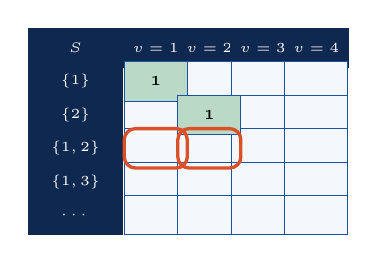
\begin{tikzpicture}[scale=0.85,
  cell/.style={draw=midblue,fill=lightblue!20,minimum width=0.8cm,minimum height=0.5cm,font=\tiny},
  hdr/.style={draw=darkblue,fill=darkblue,text=white,minimum width=0.8cm,minimum height=0.5cm,font=\tiny\bfseries}]
  % Table header
  \node[hdr,minimum width=1.2cm] at (0,2.5) {$S$};
  \foreach \v/\x in {1/1.2, 2/2.0, 3/2.8, 4/3.6}{
    \node[hdr] at (\x,2.5) {$v=\v$};}
  % Rows
  \foreach \s/\y/\lbl in {
    0/2.0/{$\{1\}$}, 1/1.5/{$\{2\}$}, 2/1.0/{$\{1,2\}$},
    3/0.5/{$\{1,3\}$}, 4/0.0/{$\cdots$}}{
    \node[hdr,minimum width=1.2cm] at (0,\y) {\lbl};
    \foreach \x in {1.2,2.0,2.8,3.6}{
      \node[cell] at (\x,\y) {};}}
  % Highlight base cases
  \node[cell,fill=dkgreen!30] at (1.2,2.0) {\textbf{1}};
  \node[cell,fill=dkgreen!30] at (2.0,1.5) {\textbf{1}};
  \node[draw=accent,very thick,rounded corners,minimum width=0.8cm,minimum height=0.5cm] at (1.2,1.0) {};
  \node[draw=accent,very thick,rounded corners,minimum width=0.8cm,minimum height=0.5cm] at (2.0,1.0) {};
\end{tikzpicture}

\vspace{0.3cm}
\textbf{Table size:} $2^n \times n$ entries\\[3pt]
\textbf{Iteration order:} by $|S|$ (increasing)\\[3pt]
\textbf{Bottleneck:} $2^{61} \times 61 \approx 1.4 \times 10^{20}$ cells
\end{center}
\end{columns}
\end{frame}

\begin{frame}{Why Ordering Matters: Frontier Width}
\small
\begin{columns}[c]
\column{0.52\textwidth}
\textbf{Key:} don't track $S$ — track connectivity on the frontier.

\vspace{0.1cm}
Process vertices in order $\sigma=(v_1,\ldots,v_n)$.
At step $i$, the \textbf{frontier} is:
\[
  F_i = \{v_j : j \le i,\;\exists\,k > i,\;(v_j, v_k) \in E\}
\]
vertices introduced but still having future neighbours.

\vspace{0.1cm}
\begin{block}{State reduction}
  Two configurations are \emph{equivalent} if they induce
  the same connectivity pattern on the frontier.\\[2pt]
  States at step $i$: at most $\Bell(|F_i|)$.
\end{block}

\column{0.44\textwidth}
\centering
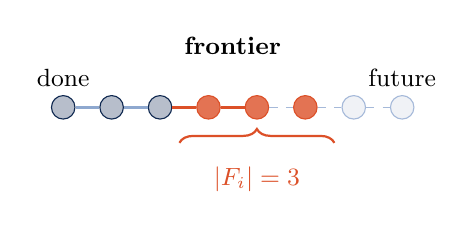
\begin{tikzpicture}[scale=0.82,
  done/.style={fill=darkblue!30,draw=darkblue,circle,inner sep=3pt},
  front/.style={fill=accent!80,draw=accent,text=white,circle,inner sep=3pt},
  future/.style={fill=lightgray,draw=midblue!40,circle,inner sep=3pt},
  lbl/.style={font=\small}]
  \foreach \x/\s in {0/done,1/done,2/done,3/front,4/front,5/front,6/future,7/future}{
    \node[\s] (\x) at (\x*0.75,0) {};}
  \draw[very thick,midblue!50] (0)--(1)--(2);
  \draw[very thick,accent] (2)--(3) (3)--(4);
  \draw[dashed,midblue!40] (4)--(5) (5)--(6) (6)--(7);
  \node[lbl,above=4pt] at (0) {done};
  \node[lbl,above=4pt] at (3.5*0.75,0.5) {\textbf{frontier}};
  \node[lbl,above=4pt] at (7*0.75,0) {future};
  \draw[decorate,decoration={brace,amplitude=5pt},thick,accent]
    (2.4*0.75,-0.55) -- (5.6*0.75,-0.55) node[midway,below=5pt]{\small $|F_i| = 3$};
\end{tikzpicture}

\vspace{0.35cm}
\textbf{Crucial:} the frontier width $|F_i|$ depends entirely on the ordering $\sigma$.\\[4pt]
Choose $\sigma$ to \alert{minimise $\max_i |F_i|$}\\
and the state space shrinks dramatically.
\end{columns}
\end{frame}

\begin{frame}{Pruning States That Cannot Finish \hfill{\normalsize after Zhao Hui Du}}
\footnotesize
\begin{columns}[t]
\column{0.52\textwidth}
Zhao Hui Du's program \texttt{path4.cpp} (emathgroup, GitHub) discards a
partial state once the unfinished vertices can no longer be joined into
one path. The plain frontier DP keeps such a state until the last step.

\vspace{0.1cm}
\textbf{After step $i<n-1$:} $F$ = frontier, $U$ = vertices still to
come, $N\subseteq F$ = frontier vertices of degree $<2$.
$H_\sigma$ = edges of $G$ inside $U$ and between $N$ and $U$, plus a link
joining the two frontier ends of each chain.

\vspace{0.1cm}
\begin{block}{Proposition (necessary for completion)}
\begin{itemize}
  \item[(C)] $H_\sigma$ is connected and $N\neq\emptyset$;
  \item[(D)] \emph{endpoint budget:} the vertices forced to be path ends
    number at most $2$:\\
    chains whose other end has left $F$,\\
    $u\in F$ of degree $0$ with one neighbour in $U$,\\
    $w\in U$ of degree $1$ in $H_\sigma$.
\end{itemize}
\end{block}

\column{0.44\textwidth}
\textbf{Why it is safe:} a Hamiltonian path completing $\sigma$, with each
chain replaced by its link, is a spanning path of $H_\sigma$ (C), and has
exactly two ends (D). Dropping violators leaves the count unchanged
(also for cycles).

\vspace{0.15cm}
\textbf{Simplest dead state:} three chains whose other ends have left the
frontier: no path has three ends.

\vspace{0.15cm}
\begin{exampleblock}{How much is dead?}
\begin{itemize}
  \item $n=52$: \textbf{55\%} of all states
  \item all fail (D); (C) never adds anything here
\end{itemize}
The unpruned table also holds every successor of an earlier dead state:
at $n=61$, \textbf{4.4$\times$} fewer states in total and the DP is
\textbf{4.2$\times$} faster (1177\,s $\to$ 282\,s, M3 Pro laptop).
\end{exampleblock}
\end{columns}
\end{frame}

% ==================== PART III: BELL / PATHWIDTH ====================
{
\setbeamercolor{background canvas}{bg=darkblue}
\begin{frame}[plain]
  \vspace{2cm}
  \begin{center}
    {\color{lightblue}\small Part III}\\[0.4cm]
    {\color{white}\LARGE\bfseries Bell Numbers and Pathwidth}
  \end{center}
\end{frame}
}

\begin{frame}{Bell Numbers: Why They Determine Complexity}
\small
\begin{columns}[c]
\column{0.50\textwidth}
\begin{block}{Definition}
$\Bell(w)$ = number of partitions of a set of $w$ elements.\\[3pt]
Equivalently: number of distinct connectivity patterns
on a frontier of width $w$ in a Hamiltonian path DP.
\end{block}

\vspace{0.2cm}
\begin{center}
\begin{tabular}{rr@{\hskip 8pt}l}
\toprule
$w$ & $\Bell(w)$ & note \\
\midrule
 8 &          4{,}140 & \\
 9 &         21{,}147 & \\
10 &        115{,}975 & $\pw(G_{57}) = 11$ \\
11 &        678{,}570 & \\
12 &      4{,}213{,}597 & $\pw(G_{58}) = 12$ \\
13 &     27{,}644{,}437 & $\pw(G_{59,60}) = 13$ \\
\rowcolor{accent!10}
14 & 190{,}899{,}322 & $\pw(G_{61}) = 14$ \\
\bottomrule
\end{tabular}
\end{center}

\column{0.46\textwidth}
\textbf{Super-exponential growth:}
\[
  \Bell(w+1) \approx \frac{w}{\ln w} \cdot \Bell(w)
\]

\vspace{0.1cm}
\begin{center}
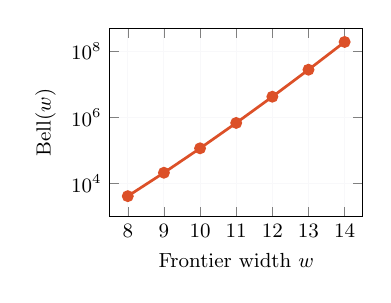
\begin{tikzpicture}[scale=0.82]
  \begin{axis}[
    xlabel={Frontier width $w$},
    ylabel={$\Bell(w)$},
    ymode=log,
    xtick={8,9,10,11,12,13,14},
    xmin=7.5, xmax=14.5,
    ymin=1000, ymax=500000000,
    width=5.5cm, height=4.5cm,
    grid=both, grid style={lightgray!50},
    tick label style={font=\small},
    label style={font=\small}]
  \addplot[accent,mark=*,mark size=2pt,very thick] coordinates {
    (8,4140)(9,21147)(10,115975)(11,678570)
    (12,4213597)(13,27644437)(14,190899322)};
  \end{axis}
\end{tikzpicture}
\end{center}

\vspace{0.1cm}
{\small Each unit increase in $\pw$ multiplies the\\
state count by $\approx 5$--$7\times$.\\
$\pw = 13 \to 14$: \textbf{$6.9\times$ more states}.}
\end{columns}
\end{frame}

\begin{frame}{Vertex Separation and Pathwidth}
\small
\begin{columns}[c]
\column{0.52\textwidth}
\begin{block}{Pathwidth (Robertson-Seymour, 1983)}
\[
  \pw(G) = \min_{\sigma} \max_{i}\, |F_i(\sigma)|
\]
Min possible max frontier width over all orderings $\sigma$.
\end{block}

\vspace{0.1cm}
\textbf{Vertex separation:} min vertices simultaneously
``in play'' sweeping $G$ left to right.

\vspace{0.1cm}
\begin{exampleblock}{For square-sum graphs: $\pw(G_{57})=11$, $\pw(G_{58})=12$, $\pw(G_{59,60})=13$, $\pw(G_{61})=14$}
\end{exampleblock}

\column{0.44\textwidth}
\textbf{Why does pathwidth matter so sharply?}

\vspace{0.1cm}
Total DP work $\le \sum_i \Bell(|F_i(\sigma)|)$.\\
Under the optimal ordering:
\[
  \text{work} = O\bigl(\Bell(\pw(G)) \cdot n\bigr)
\]

\vspace{0.1cm}
Compare to Held-Karp: $O(2^n \cdot n)$.\\
For $n = 61$, $\pw = 14$:
\begin{align*}
  2^{61} &\approx 2.3 \times 10^{18} \\
  \Bell(14) &\approx 1.9 \times 10^8
\end{align*}

\begin{center}
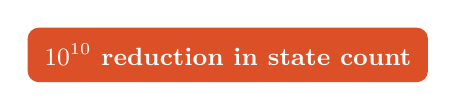
\begin{tikzpicture}
  \node[fill=accent,rounded corners,text=white,inner sep=6pt,font=\small\bfseries]{
    $10^{10}$ reduction in state count};
\end{tikzpicture}
\end{center}
\end{columns}
\end{frame}

\begin{frame}{Fixed-Parameter Tractability}
\small
\begin{columns}[c]
\column{0.52\textwidth}
\begin{block}{FPT (Downey-Fellows, 1992)}
Parameterised by $k$: solvable in $f(k)\cdot n^{O(1)}$ time,
$f$ any computable function.\\[2pt]
Combinatorial explosion \emph{confined to $k$};
for fixed $k$: polynomial in $n$.
\end{block}

\vspace{0.1cm}
\textbf{Ham.\ path counting is FPT} by pathwidth:
\[
  \text{time} = O\bigl(\underbrace{\Bell(\pw)}_{\text{f(k)}} \cdot \underbrace{n}_{\text{poly}}\bigr)
\]

\column{0.44\textwidth}
\textbf{Treewidth as an alternative parameter:}

\vspace{0.1cm}
$\tw(G) \le \pw(G)$ always. For our graphs:\
$\tw(G_{61}) \approx 11$--$12 \approx \pw - 2$.

\vspace{0.15cm}
\begin{alertblock}{Why not use treewidth?}
\begin{itemize}\small
  \item Join-node cost: $O(\Bell(\tw)^2)$ vs $O(\Bell(\pw))$ per step
  \item $\tw=11$: $\Bell(11)^2 \approx 4.6 \times 10^{11}$;\quad $\pw=14$: $\Bell(14) \approx 1.9 \times 10^8$
  \item Treewidth DP is \textbf{$2000\times$ worse} here
  \item Exact treewidth also harder to compute for these graphs
\end{itemize}
\end{alertblock}
\end{columns}
\end{frame}

% ==================== PART IV: ORDERING ====================
{
\setbeamercolor{background canvas}{bg=darkblue}
\begin{frame}[plain]
  \vspace{2cm}
  \begin{center}
    {\color{lightblue}\small Part IV}\\[0.4cm]
    {\color{white}\LARGE\bfseries Computing the Best Ordering}
  \end{center}
\end{frame}
}

\begin{frame}{Finding the Optimal Ordering: MaxSAT}
\small
\begin{columns}[c]
\column{0.52\textwidth}
\textbf{Problem:} exact pathwidth is NP-hard in general,
but tractable for graphs of this size.

\vspace{0.15cm}
\textbf{Vertex-separation encoding~[Coudert 2016]:}\\
$x_{v,i}$: ``$v$ placed at position $\le i$''.\\
Clauses: $v$ on frontier iff introduced and not yet eliminated.\\
Minimise $\max|F_i|$.

\vspace{0.1cm}
\begin{block}{Output}
Exact $\pw(G_n)$ and optimal ordering.
Enumeration mode: generator over \textbf{all} optimal-pw
orderings — enabling multi-start SA.
\end{block}

\column{0.44\textwidth}
\textbf{Enumeration timing for $n=60$:}

\vspace{0.1cm}
{\small
\begin{tabular}{rr}
\toprule
Solution & Time (s) \\
\midrule
1 (proves $\pw=13$) & 149.0 \\
2 & 5.9 \\
3 & 15.6 \\
4 & 3.1 \\
5--8 & 0.04--0.08 \\
9--60+ & $\approx 0.034$ \\
\bottomrule
\end{tabular}}

\vspace{0.2cm}
Solutions 1--4 are \textbf{structurally distinct}
(require genuine re-solving). Solutions 5+ are local
variations reachable by unit propagation — and by SA.

\vspace{0.2cm}
\begin{exampleblock}{Practical rule: stop at 10 consecutive $<$40\,ms solutions}
\end{exampleblock}
\end{columns}
\end{frame}

\begin{frame}{Simulated Annealing Refinement}
\small
\begin{columns}[c]
\column{0.52\textwidth}
\textbf{Motivation:} same $\pw(G)$, but DP costs differ by up to $50\%$.

\vspace{0.15cm}
\textbf{$G_{57}$, $\pw = 11$:}
\begin{center}\small
\begin{tabular}{lrr}
\toprule
Ordering & Time & Peak \\
\midrule
MaxSAT only & 42.7\,s & 4.6M \\
+ SA (V5) & $\approx$25\,s & 4.1M \\
\bottomrule
\end{tabular}
\end{center}

\vspace{0.1cm}
\textbf{SA design:}
\begin{itemize}
  \item Start: MaxSAT-optimal ordering
  \item Move: adjacent swap, only if $\max|F_i|$ unchanged
  \item Cost (V5): $C(\sigma)=\sum_i \hat{s}_i\cdot 2^{\nb(i)}\cdot|F_i|$
\end{itemize}

\column{0.44\textwidth}
\textbf{What SA can and cannot do:}

\vspace{0.1cm}
SA freely moves vertices that slide without changing $\max|F_i|$ — exactly the cheap ($\approx$34ms) MaxSAT solutions.

\vspace{0.15cm}
SA \textbf{cannot} cross between distinct topological skeletons without temporarily raising $\pw$.

\vspace{0.1cm}
\begin{block}{Multi-start strategy}
  SA from each of $\sim$4--8 distinct MaxSAT solutions;
  take lowest V5 cost.\\[2pt]
  {\small $n=57$: $134$\,s $\to$ $25$\,s ($\mathbf{5.4\times}$)}
\end{block}
\end{columns}
\end{frame}

\begin{frame}{New: Kobayashi's DP and a DAG of Optimal Orderings}
\scriptsize
\begin{columns}[t]
\column{0.52\textwidth}
\textbf{Relevant-set DP}~[Kobayashi 2015]: states are \emph{relevant}
vertex sets, at most $3^{\tau(G)}$ ($\tau$ = vertex cover number).
A step's cost does not depend on $k$, so $\pw(G)$ is a
\textbf{min-bottleneck path} in a DAG of sets.
\begin{itemize}
  \item \textbf{One pass}, no bound $k$ supplied; never more work than
        one decision call at $k=\pw$
  \item greedy rule of Coudert--Mazauric--Nisse: $2$--$6\times$ fewer sets
\end{itemize}

\vspace{0.05cm}
\begin{block}{Keep the whole optimal layer}
Finish the last level, prune backwards: every source-to-sink path is a
$\pw$-optimal ordering.
\begin{center}\vspace{-0.15cm}
\begin{tabular}{rrrr}
\toprule
$n$ & $\pw$ & DAG nodes & orderings \\
\midrule
57 & 11 & 13{,}762  & $1.6\cdot10^{26}$ \\
59 & 13 & 151{,}041 & $2.0\cdot10^{31}$ \\
61 & 14 & 263{,}672 & $2.2\cdot10^{33}$ \\
\bottomrule
\end{tabular}
\end{center}
\vspace{-0.15cm}
{\tiny A strict subfamily of all optimal orderings (block boundaries
at relevant sets); for $n\le35$ the V2 optimum over it is within
$0.3$--$1.7\%$ of the global one.}
\end{block}

\column{0.44\textwidth}
\textbf{Exact secondary optimisation.}
Each DP step adds $a+p\,e$ to the cost and multiplies the carried
state proxy $p$ by $e\,k$. A Pareto-label DP over (cost, $p$) finds the
\textbf{exact} optimum over the whole DAG: no annealing, no multi-start.

\vspace{0.05cm}
{\tiny Label caps $64,512,4096,\infty$ with a time budget; the
result is reported as certified or truncated.}

\vspace{0.05cm}
\begin{exampleblock}{$n=75$, ordering time}
\begin{tabular}{lr}
MaxSAT + SA (April) & $2179$\,s \\
pathwidth (kpw) & $0.8$\,s \\
+ exact work-model optimum & $22$\,s \\
\end{tabular}
\end{exampleblock}

\vspace{0.05cm}
\textbf{The choice still matters:} over 12 optimal orderings per $n$
($50\le n\le56$) total states vary $1.4$--$3.0\times$. At $n=75$ the V7
optimum needed $24\%$ fewer states than the work-model optimum.

\vspace{0.05cm}
{\tiny Details: V.~Miller, \emph{One-pass bottleneck search for
linear width parameters} (in preparation).}
\end{columns}
\end{frame}

% ==================== PART V: PRACTICAL ====================
{
\setbeamercolor{background canvas}{bg=darkblue}
\begin{frame}[plain]
  \vspace{2cm}
  \begin{center}
    {\color{lightblue}\small Part V}\\[0.4cm]
    {\color{white}\LARGE\bfseries Practical Computation}
  \end{center}
\end{frame}
}

\begin{frame}{The Record-Merging Bottleneck}
\small
\begin{columns}[c]
\column{0.52\textwidth}
At each DP step: large set of \textbf{(state, count)} pairs.

\vspace{0.15cm}
\textbf{Merging requirement:}\\
Many source states $\to$ same output state.
Counts must be \textbf{summed}:
\[
  \texttt{nxt}[k] \mathrel{+}= c_A + c_B + \cdots
\]
A \textbf{record-merging problem}: stream of (key, value) pairs,
deduplicate and aggregate.

\vspace{0.15cm}
\textbf{Scale at $n=61$:}
\begin{itemize}
  \item Peak: $619$M output states
  \item 24 bytes each (8B key + 16B count)
  \item Peak table: $\approx 20$\,GB live
\end{itemize}

\column{0.44\textwidth}
\begin{alertblock}{The engineering problem}
  Requires attention to the \textbf{storage hierarchy}:
  L1, L2, L3, DRAM, swap.\\[3pt]
  \textbf{Subject of Talk II.}\\[3pt]
  Short version: LP hash table (infeasible at $n=61$)
  $\to$ extendible hashing + radix-sort locality +
  OS page reclaim. Peak memory: $>80$\,GB $\to$ $<2$\,GB.
\end{alertblock}

\vspace{0.15cm}
{\small $n=61$: 97\,min on M3 Pro.
Without Talk II engineering: killed by OS.\\
Now, with pruning: 282\,s (M3 Pro laptop).}
\end{columns}
\end{frame}

\begin{frame}{Competing Approaches}
\small
\begin{columns}[t]
\column{0.30\textwidth}
\begin{block}{ZDD / Graphillion}
  Zero-suppressed BDDs represent path sets as DAGs.\\[3pt]
  \textbf{Pro:} Elegant, general\\[2pt]
  \textbf{Con:} ZDD size explodes; exhausted 16\,GB at $n \le 56$
\end{block}

\column{0.30\textwidth}
\begin{block}{Held-Karp directly}
  $O(2^n \cdot n)$ DP on the full visited-set table.\\[3pt]
  \textbf{Pro:} Simple, optimal for general graphs\\[2pt]
  \textbf{Con:} $2^{61}$ states $\approx 10^{18}$\\
  — completely infeasible
\end{block}

\column{0.30\textwidth}
\begin{block}{Inclusion-exclusion (Giscard)}
  Sum over connected dominating sets.\\[3pt]
  \textbf{Pro:} Theoretically clean\\[2pt]
  \textbf{Con:} $|\text{CDS}(G_n)| \approx 3^n$;\\
  $\approx 4 \times 10^{29}$ terms for $n = 61$
\end{block}
\end{columns}

\vspace{0.15cm}
\begin{center}
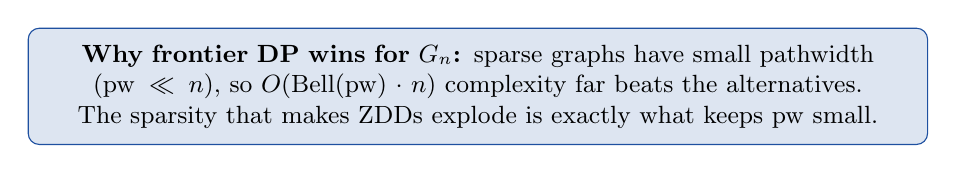
\begin{tikzpicture}
\node[fill=midblue!15,draw=midblue,rounded corners,inner sep=6pt,text width=11cm,align=center,font=\small]{
  \textbf{Why frontier DP wins for $G_n$:} sparse graphs have small pathwidth ($\pw \ll n$),
  so $O(\Bell(\pw) \cdot n)$ complexity far beats the alternatives.
  The sparsity that makes ZDDs explode is exactly what keeps $\pw$ small.};
\end{tikzpicture}
\end{center}
\end{frame}

% ==================== RESULTS ====================
{
\setbeamercolor{background canvas}{bg=darkblue}
\begin{frame}[plain]
  \vspace{2cm}
  \begin{center}
    {\color{lightblue}\small Part VI}\\[0.4cm]
    {\color{white}\LARGE\bfseries New Results}
  \end{center}
\end{frame}
}

\begin{frame}{New Values: $|\mathrm{Ham}(G_n)|$ for $n\le 75$}
\footnotesize
\begin{columns}[t]
\column{0.50\textwidth}
\centering
{\scriptsize
\renewcommand{\arraystretch}{0.9}
\begin{tabular}[t]{rrr}
\toprule
$n$ & $\pw$ & $|\mathrm{Ham}(G_n)|$ \\
\midrule
57 & 11 & 68{,}092{,}497{,}615 \\
58 & 12 & 123{,}092{,}214{,}818 \\
59 & 13 & 332{,}409{,}010{,}079 \\
60 & 13 & 783{,}175{,}077{,}980 \\
61 & 14 & 3{,}711{,}439{,}128{,}718 \\
62 & 14 & 19{,}133{,}360{,}717{,}991 \\
63 & 14 & 121{,}460{,}168{,}051{,}419 \\
64 & 14 & 329{,}054{,}896{,}751{,}390 \\
65 & 14 & 780{,}444{,}607{,}816{,}976 \\
66 & 14 & 1{,}389{,}466{,}102{,}344{,}323 \\
67 & 14 & 2{,}317{,}807{,}210{,}864{,}530 \\
68 & 14 & 5{,}019{,}822{,}900{,}252{,}036 \\
69 & 14 & 6{,}697{,}388{,}275{,}608{,}246 \\
70 & 14 & 12{,}684{,}480{,}251{,}402{,}254 \\
71 & 14 & 65{,}830{,}124{,}660{,}217{,}873 \\
72 & 14 & 132{,}407{,}660{,}925{,}860{,}729 \\
73 & 14 & 536{,}884{,}024{,}745{,}221{,}467 \\
74 & 14 & 2{,}176{,}025{,}661{,}130{,}535{,}741 \\
\rowcolor{dkgreen!15}
75 & 15 & \textbf{9{,}231{,}885{,}593{,}047{,}053{,}408} \\
\bottomrule
\end{tabular}}

\column{0.46\textwidth}
\textbf{Width:} $\pw$ rises $13\to14$ at $n=61$ and $14\to15$ at
$n=75$; the state count is governed by $\pw$, not by $n$.

\vspace{0.1cm}
\textbf{Later gains:} storage engineering (Talk~II), pruning dead
states ($4.2\times$ at $n=61$), and orderings optimised exactly over the
Kobayashi DAG.

\vspace{0.1cm}
\begin{block}{Checks}
{\scriptsize $n=75$: two different optimal orderings give the same count
(an earlier value, from a run with too few key slots, is withdrawn).
All values are computed modulo $2^{64}$ with CRT replay when a count wraps.}
\end{block}
\end{columns}
\end{frame}

\begin{frame}{Key Insight Cascade}
\vspace{0.1cm}
\begin{center}
{\small
\colorbox{lightblue!40}{\parbox{0.88\textwidth}{\centering\vspace{3pt}
  \textbf{Counting Hamiltonian paths is \#P-complete.}\\[1pt]
  But $G_n$ is sparse with small pathwidth $\pw \ll n$.
\vspace{3pt}}}

\vspace{1pt}{\color{midblue}$\downarrow$}\vspace{1pt}

\colorbox{midblue!20}{\parbox{0.88\textwidth}{\centering\vspace{3pt}
  \textbf{Frontier DP reduces Held-Karp's $O(2^n)$ to $O(\Bell(\pw))$ states.}\\[1pt]
  Bell numbers grow super-exponentially: each unit of $\pw$ costs $6$--$7\times$.
\vspace{3pt}}}

\vspace{1pt}{\color{midblue}$\downarrow$}\vspace{1pt}

\colorbox{accent!15}{\parbox{0.88\textwidth}{\centering\vspace{3pt}
  \textbf{Kobayashi's DP gives the exact $\pw$ and a DAG of optimal orderings.}\\[1pt]
  A secondary cost is minimised exactly over $\ge10^{26}$ optimal orderings, in seconds.
\vspace{3pt}}}

\vspace{1pt}{\color{midblue}$\downarrow$}\vspace{1pt}

\colorbox{dkgreen!15}{\parbox{0.88\textwidth}{\centering\vspace{3pt}
  \textbf{At scale, the record-merging step dominates.}\\[1pt]
  Storage-aware engineering plus pruning reaches $n=75$ (17\,min DP, 64 cores).\\[1pt]
  Without it, the computation would exhaust RAM and never complete.
\vspace{3pt}}}
}
\end{center}
\end{frame}

% ==================== FINAL ====================
{
\setbeamercolor{background canvas}{bg=darkblue}
\begin{frame}[plain]
  \vspace{0.5cm}
  \begin{center}
    {\color{white}\Large\bfseries Thank You}\\[0.5cm]
    {\color{lightblue}Questions?}\\[0.6cm]

    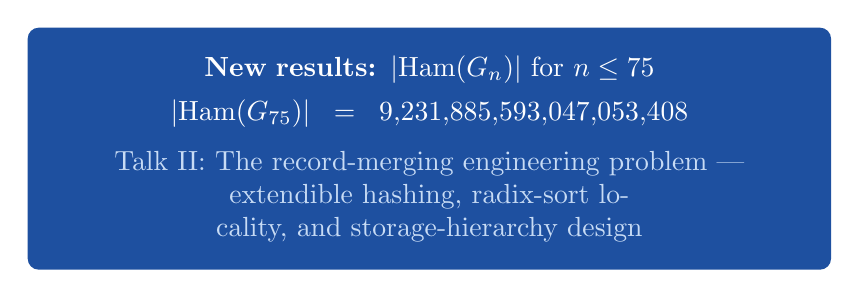
\begin{tikzpicture}
    \node[fill=midblue,rounded corners,inner sep=10pt,text=white,
          text width=9.5cm,align=center]{
      \textbf{New results:} \mbox{$|\mathrm{Ham}(G_n)|$ for $n\le 75$}\\[4pt]
      $|\mathrm{Ham}(G_{75})| = 9{,}231{,}885{,}593{,}047{,}053{,}408$\\[6pt]
      \textcolor{lightblue}{Talk II: The record-merging engineering problem —\\
      extendible hashing, radix-sort locality, and storage-hierarchy design}};
    \end{tikzpicture}

    \vspace{0.5cm}
    {\color{lightblue!70}\small
    With thanks to Claude (Anthropic) for algorithm design, profiling, and implementation.}
  \end{center}
\end{frame}
}

\end{document}
